\section{Laboratory Lecture 2: Safe Code}

The aim of this laboratory session is to build a basic access control system. To do this, an ATMega328P will be used, as per the previous lecture, in combination with a 16x2 LCD display, in order to show the different messages, and a keypad, to allow the user to enter the security code.\medskip

The correct password will be stored in the \textbf{EEPROM}, a type of memory that will be discussed later. A relay connected to the system, will be triggered when the correct password is entered.

\subsection{Introduction}

Three main components will be used in this laboratory session, namely an Arduino UNO, which packs an ATMega328P, a 3x4 Keypad, and a 16x2 LCD display. The Arduino board was introduced in the last practice, see \textbf{Subsection \ref{sec:ARDUINO}} for more on this topic. The same can be said about the keypad, which was also introduced in a previous VHDL laboratory lesson, \textbf{see Subsubsection \ref{sec:KEYPAD}} for more on this topic. To read the key presses, we will use a C library, which will be discussed later.\medskip

A brief introduction to the 16x2 LCD display is necessary to fully understand the session.

\subsubsection{16x2 LCD Display}

In previous practices we have used 7-segment displays to show information. This displays, though useful, cannot show text messages, and, in general, take a lot of space. LCD technology has been around for a lont time now, and because of this, the cost of panels has become significantly cheaper over the years. \medskip

Nowadays, 16x2 or 16x4 LCD are readily available and can be found in most electronic kits. They allow the user to display complex alphanumerical messages without a hassle.\medskip

An image of the 16x2 LCD that we will use in this practice can be found below:

\begin{figure}[H]
    \centering
    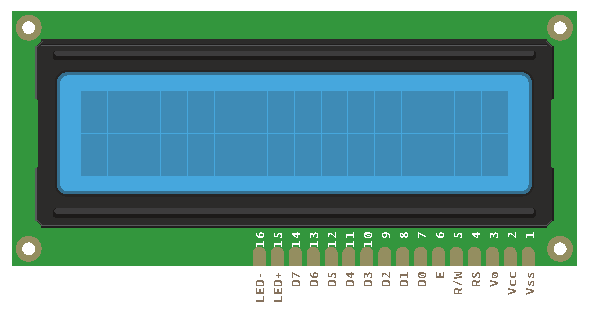
\includegraphics[scale = 0.9]{Graphics/MICROS/Practice 2/LCD.pdf}
    \caption{16x2 LCD Display~\autocite{ARDUINO}}
    \label{fig:LCD_DISPLAY}
\end{figure}

As we can see, these displays have lots of data lines, which must be connected to our microcontroller either directly, or through an I2C breakout board. The latter offers the benefit of having less data lines, 4 in this case, though a different communication protocol must be used. \medskip

In this laboratory session we will connect the display to the ATMega328P directly, following this pin configuration:

\begin{itemize}
    \item VDD  $\rightarrow$ VCC
    \item VSS  $\rightarrow$ GND
    \item VEE  $\rightarrow$ Potentiometer (Contrast control)
    \item RW   $\rightarrow$ PB0
    \item RS   $\rightarrow$ PD7
    \item EN   $\rightarrow$ PB1
    \item D4   $\rightarrow$ PB2
    \item D5   $\rightarrow$ PB3
    \item D6   $\rightarrow$ PB4
    \item D7   $\rightarrow$ PB5
    \item LED$+$ $\rightarrow$ VCC
    \item LED$-$ $\rightarrow$ GND
\end{itemize}

The rest of the pins will be left floating, since we will use 4-bit mode.\medskip


\clearpage

In order to interact with the display, a library will be used to simplify things. Some of the basic functions are explained below:

\inputCcode{CODES/MICROS/Practice_2/EXPLANATION/LCD_COMMANDS.c}

\clearpage

\subsubsection{3x4 Keypad}

The keypad was introduced in a previous VHDL practice,\textbf{see Subsubsection \ref{sec:KEYPAD}} for more on this topic, in which a Ring Counter was used to cycle a logic 1 though the L$\left[3...0\right]$ pins. When the user pressed a key, the GAL would read the C$\left[2...0\right]$ pins in order to determine the corresponding column and by knowing the position of the 1 in the L$\left[3...0\right]$ vector, it would determine which of the 12 possible buttons was pressed by the user.\medskip

As we said before, in order to interface with the keypad in this laboratory session we will use a custom-made C library, which will help us simplify the program.\medskip

As per the LCD, the function that we must call to obtain the pressed key can be found below:

\inputCcode{CODES/MICROS/Practice_2/EXPLANATION/KEYPAD_LIBRARY.c}

\clearpage

\subsubsection{EEPROM}

As we said before, our system will compare the introduced password with a master password which will be permanently stored in the ATMega328P's EEPROM. \medskip

The EEPROM, which stands for Electrically Erasable Programmable Read-Only Memory, is a type of non-volatile memory, i.e. it maintains the stored data when no power is applied to it.\medskip

In the case of the ATMega328P, the internal EEPROM has a size of 1 KB, which is nothing compared to the 32 KB of flash memory. \medskip

The main disadvantage of this type of memory is, apart from its size, its reading/writing speeds. A writing cycle of one cell (byte) takes up to 3.3 ms. A reading cycle of 1024 bytes, though quicker at around 0.3 ms, is still slower than the built-in SRAM. Besides, these type of memories cannot be reprogrammed an infinite number of times, as they deteriorate with each writing cycle.\medskip

To interface with it, we will again use a library. An explanation of its most important functions can be found below:

\inputCcode{CODES/MICROS/Practice_2/EXPLANATION/EEPROM.c}


\subsection{Exercise 1: Safe Code}

Now that every needed component has been explained, we will move on to solving the proposed exercise.\medskip

The proposed code can be found below:

\inputCcode{CODES/MICROS/Practice_2/PRACTICE/SAFECODE.c}

\clearpage

\noindent In order to explain the code we will divide it in sections:

\begin{enumerate}
    \item The master password is saved in the EEPROM.
    \item The I/O is initialized.
    \item In the main loop, the uC checks for a keypress that is different from FF (No keypress) and it saves it in the variable keyarr[n]. At the same time, the entered numbers are displayed on the LCD. When the user has entered 3 numbers the loop ends.
    \item The content of the EEPROM is dumped into a variable.
    \item If the keyarr[n] matches the EEPROM dump, the message \textit{CORRECT} is displayed and both the relay and the LED are triggered. Otherwise, the message \textit{INCORRECT} is shown. 
    \item The program restarts.
\end{enumerate}

After compiling the code, we can simulate it in ISIS Proteus. The following animation shows the cycle that we have just described:

\begin{figure}[H]
    \centering
 
    \ifnum\value{ANIMATION}=1 {
        \animategraphics[controls,loop,scale=0.75]{1}{Graphics/MICROS/Practice 2/ANIMATION/F}{0}{9}
    } 
    \else {
        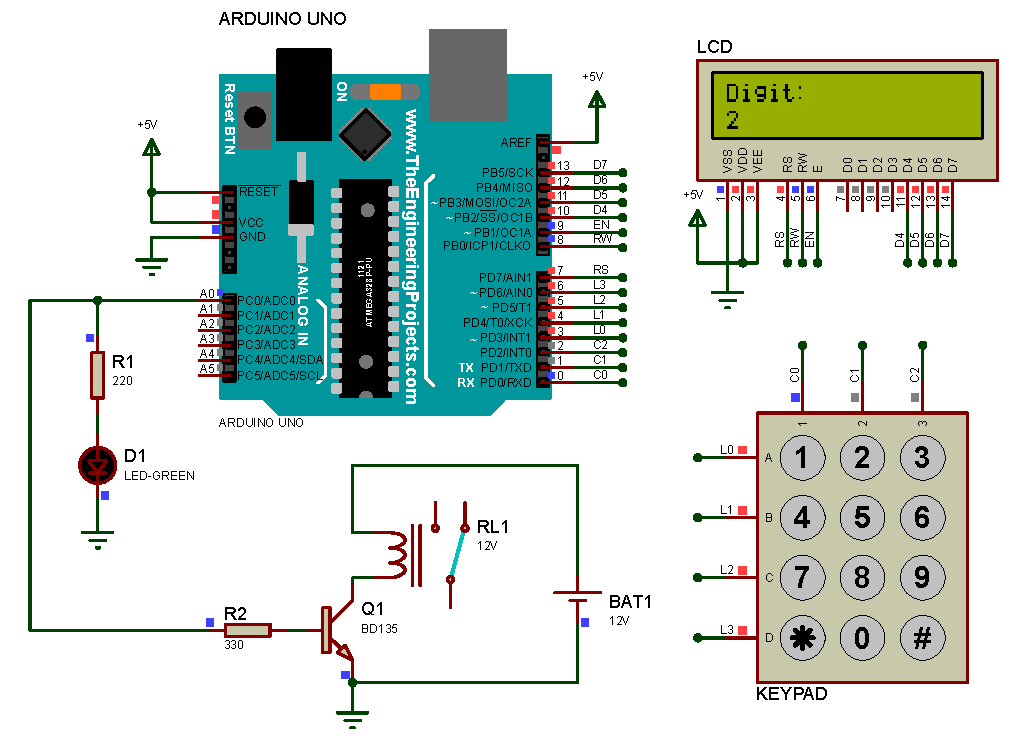
\includegraphics[scale=0.75]{Graphics/MICROS/Practice 2/ANIMATION/F2.pdf}
    }\fi
    
    \caption{Proteus Simulation}
    \label{fig:SAFECODE_PROTEUS_MICROS}
\end{figure}


\clearpage





























